Typographic correction module receives the message with the structure given by the preprocessing module and detects the typographic errors present in the given e-mail. As it is shown in Figure \ref{fig:umltypo}, this UML package has four different UML classes: \textit{TypoCorrectorApp}, \textit{TypoCorrector}, \textit{CorrectedMessage} and \textit{Correction}.

\begin{figure}[p]
	\centering%
	\centerline{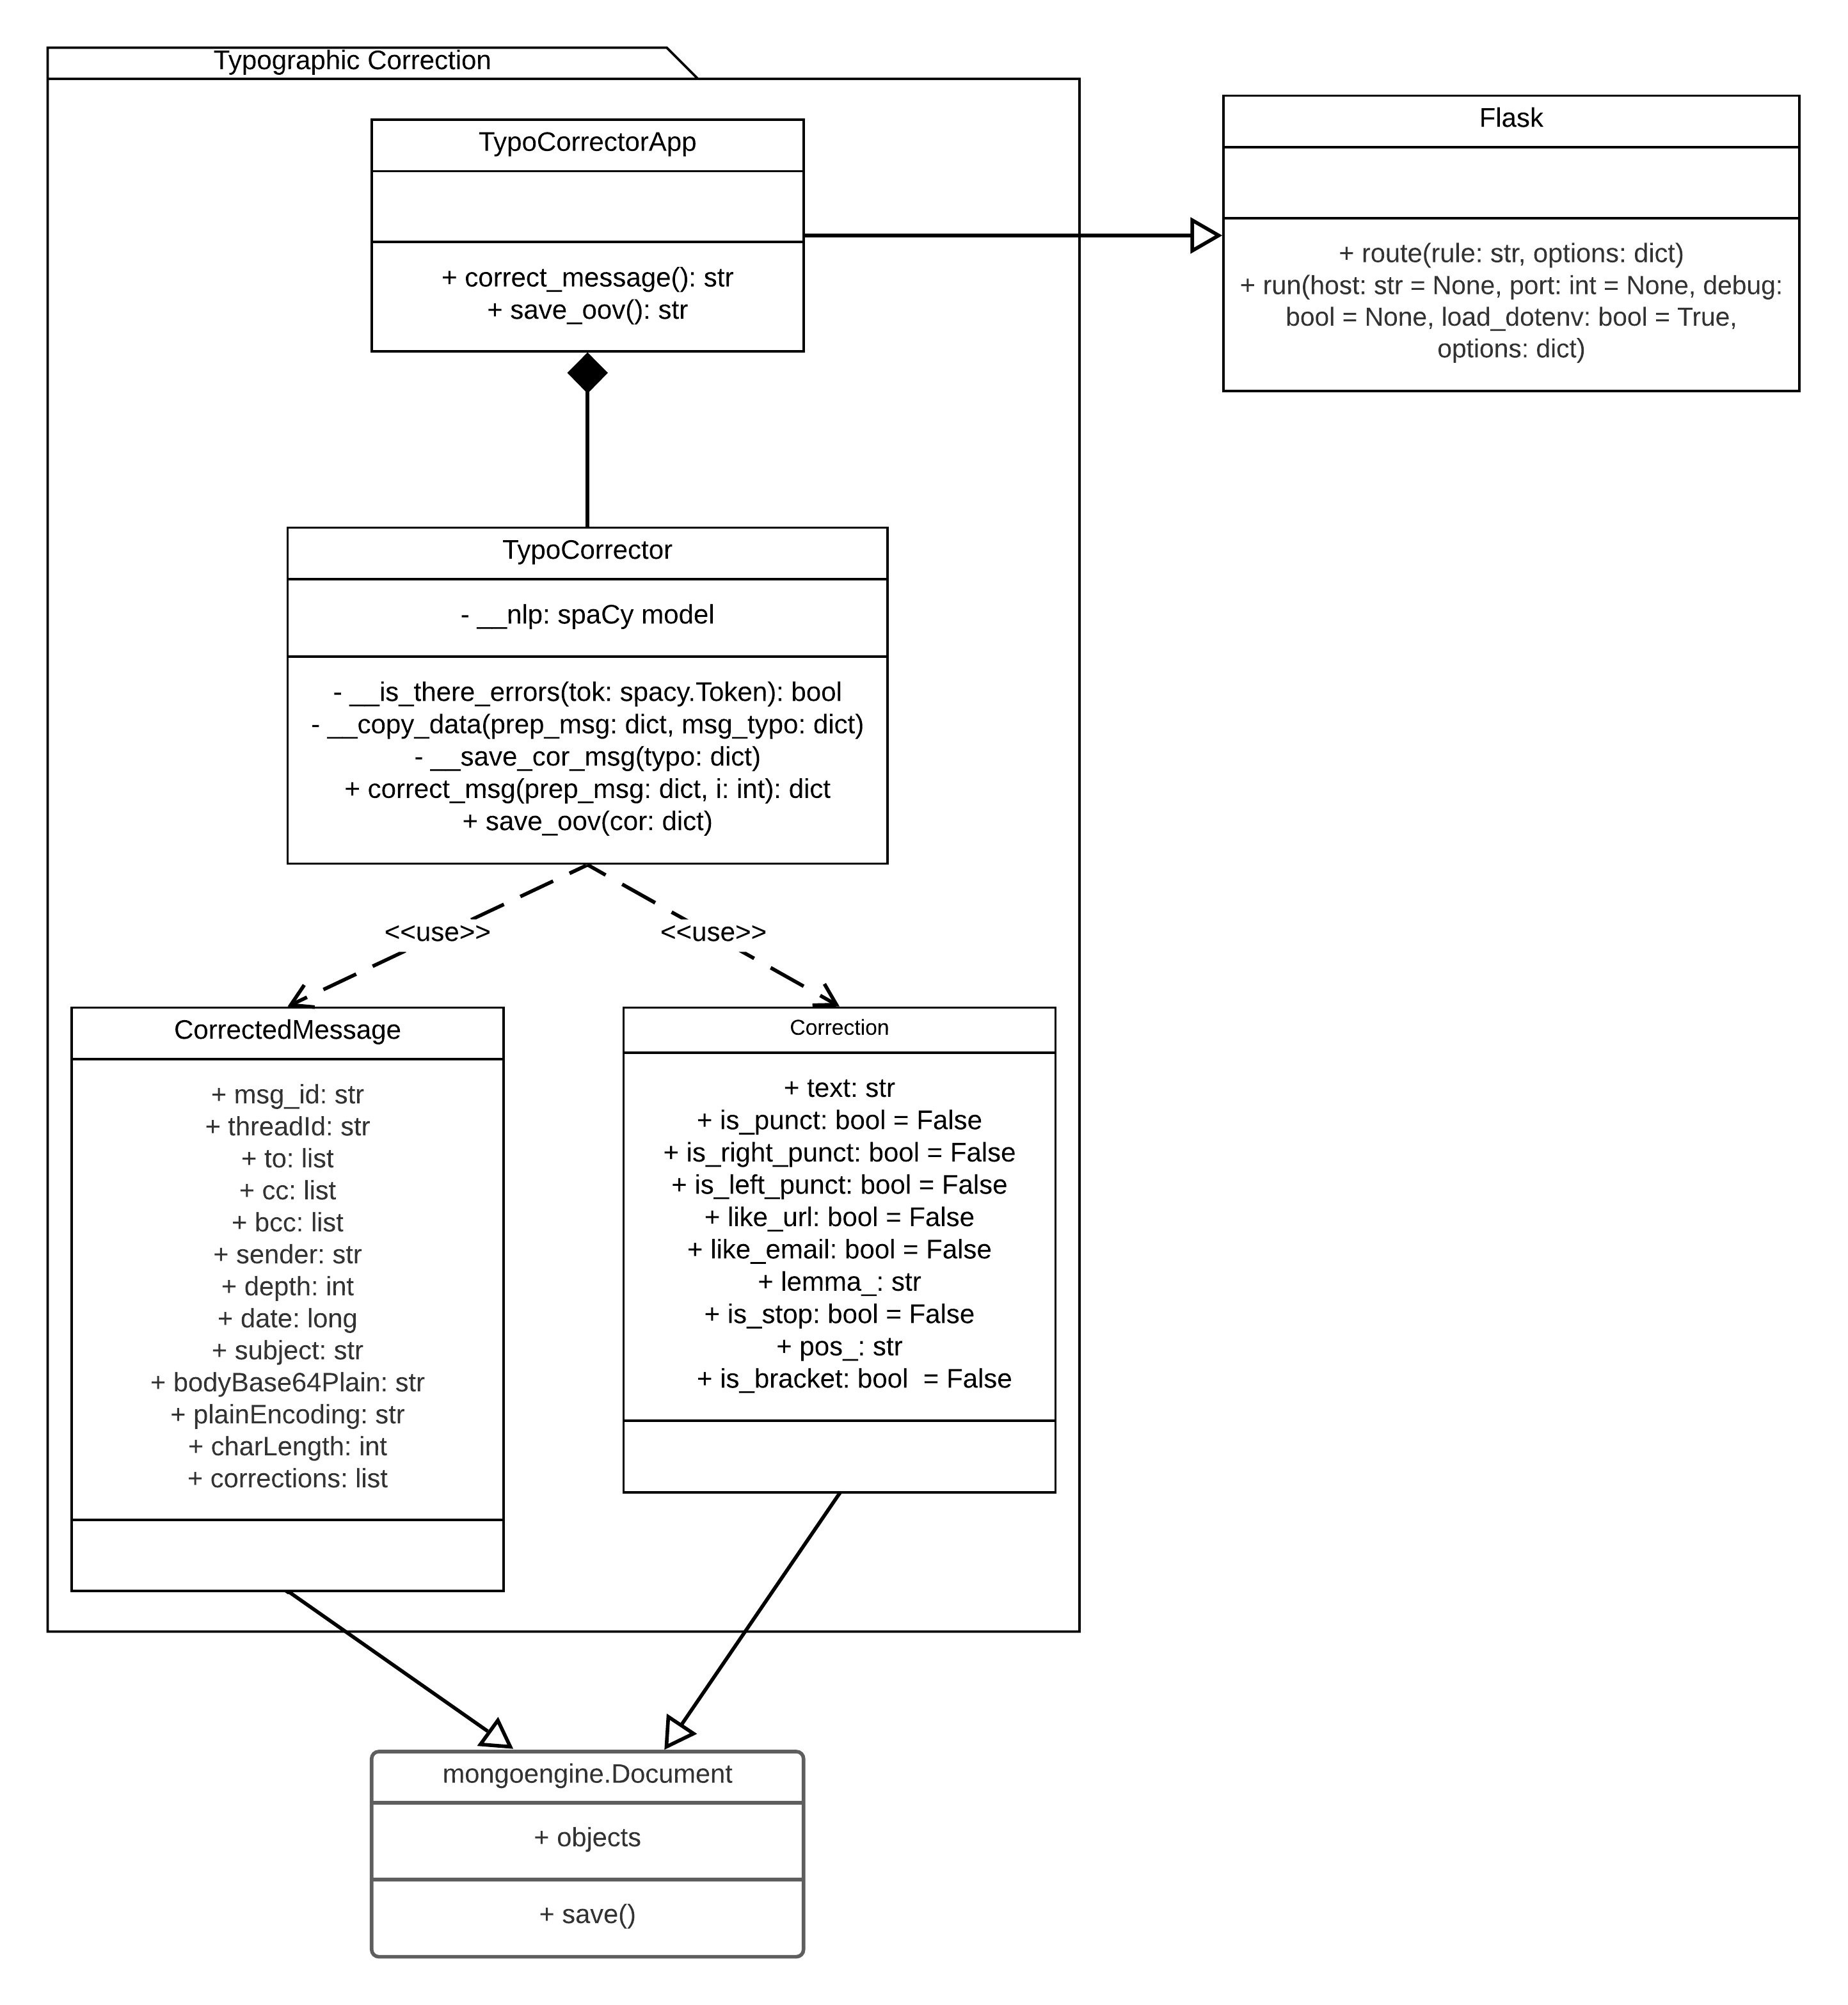
\includegraphics[width=0.9\paperwidth]{Imagenes/Bitmap/typoUML.png}}%
	\caption{UML class diagram of the typographic correction module}%
	\label{fig:umltypo}
\end{figure}

As it happened with \textit{PreprocessorApp}, \textit{TypoCorrector} inherits from \textit{Flask} class and, thanks to it, this class implements a simple web service. However, unlike \textit{PreprocessorApp}, \textit{TypoCorrector} has two different methods which carry out distinct task. These two functions correspond to the two \textit{TypoCorrector}'s public method with the same name. Thus, if we want to invoke one of these public methods, it will be necessary to execute a POST HTTP request with an e-mail, in order to be corrected (in the case of the method \textit{correct\_msg}), or with the unrecognised token (which has been wrongly classified as ``out of vocabulary'' by our spaCy's model) that is going to be saved (we will explained both tasks in detail later). Each one of them is going to have a different url address.

The main class of this UML package, as it happens with the rest of packages, is the \textit{TypoCorrector} class. It is in charge of detecting the typographic errors and correcting them if it is possible. For this purpose it makes use (as an attribute) of an spaCy's pretrained model, specifically the one called \textit{es\_core\_news\_md}\footnote{\url{https://spacy.io/models/es}}.

The first public method that we are going to explain is \textit{correct\_msg}, which receives as parameters a message and an index.